\documentclass[12pt,a4paper]{article}
\usepackage[utf8]{inputenc}
\usepackage[english]{babel}
\usepackage{amsmath}
\usepackage{amsfonts}
\usepackage{amssymb}
\usepackage{graphicx}
\usepackage{epstopdf}

\usepackage{fullpage}

\usepackage{float}

\begin{document}

\section{Pathplanning using RRT in RobWorks}
For this project, the RRT planner in RobWorks was used.
Here the path was planned from and to the two given configurations $q_{pick}$ and $q_{place}$ in the given scene.
In order to optimize the epsilon of the path planner, this was tested with respect to the time it takes to compute the path and path travelled by the tool frame.

Since the RRT planner is a probabilistic approach to finding a path between the two configurations, then the path was computed 30 times.
The data gathered for the timing of the algorithm can be seen in figure \ref{fig:timeVSepsilon} and the distance travelled by the tool in figure \ref{fig:distVSepsilon}.
To find a solution the path planner must be able to find a path within 15 seconds.
From figure \ref{fig:successfulVSepsilon} it can be seen that a low epsilon decreases the chances of finding a valid path.

% remember to remove 0 from the files (overextended timing periode)
\begin{figure}[H]
\centering
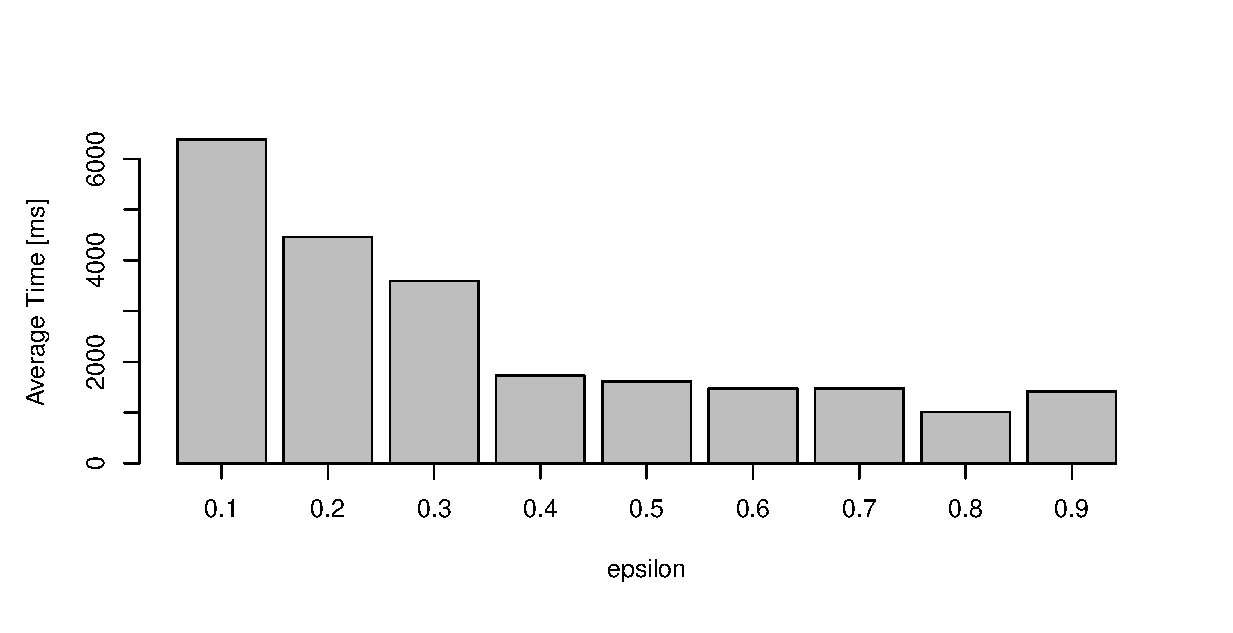
\includegraphics[width=0.7\textwidth]{../statistics/timeVSepsilon}
\caption{figure of time vs epsilon}
\label{fig:timeVSepsilon}
\end{figure}


\begin{figure}[H]
\centering
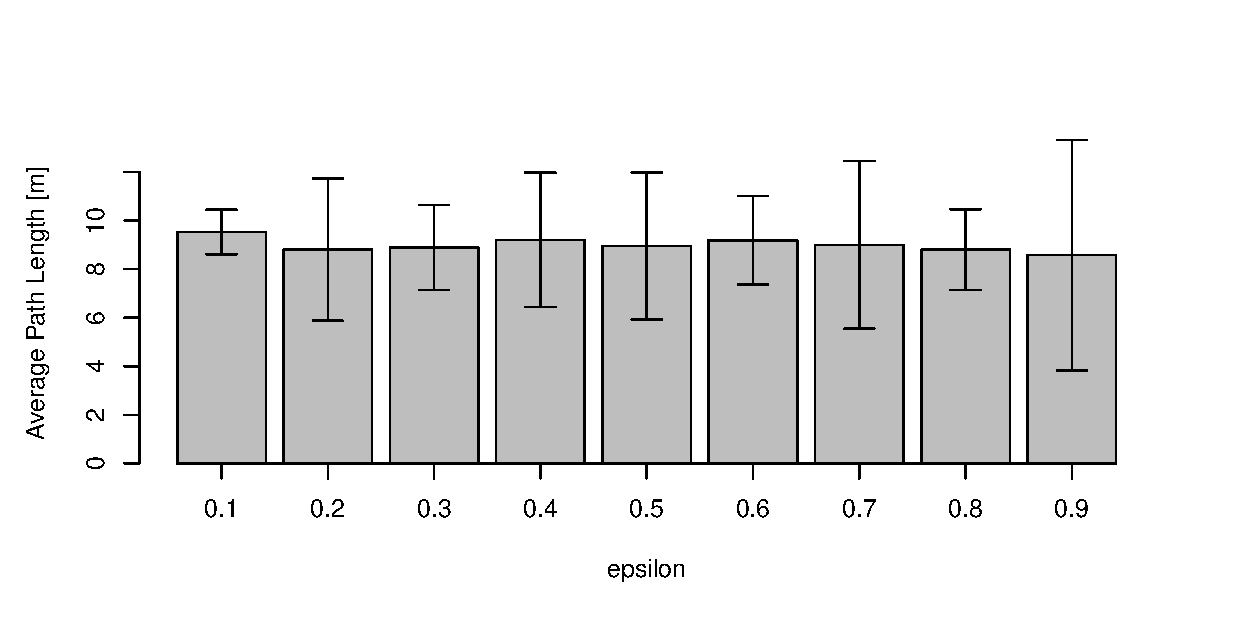
\includegraphics[width=0.7\textwidth]{../statistics/distVSepsilon}
\caption{figure of tool-frame path length vs epsilon}
\label{fig:distVSepsilon}
\end{figure}

\begin{figure}[H]
\centering
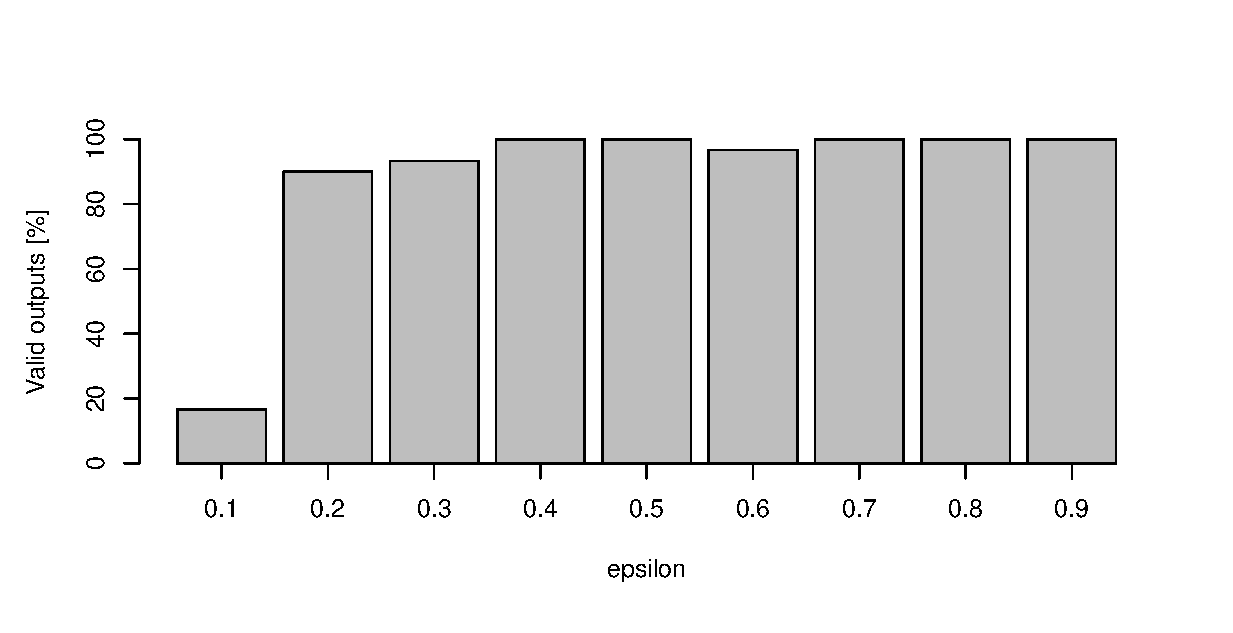
\includegraphics[width=0.7\textwidth]{../statistics/successfulVSepsilon}
\caption{figure of successful attempts within the 15 second time limit vs epsilon}
\label{fig:successfulVSepsilon}
\end{figure}


\end{document}